\documentclass{report}[12pt]
\usepackage{amssymb}
\usepackage{amsmath}
\usepackage{geometry}
\usepackage{cite}
\usepackage[utf8]{inputenc}
\usepackage{graphicx}
\graphicspath{ {images/} }
\usepackage{float}
\usepackage{listings}
\usepackage[dvipsnames]{xcolor}
\usepackage{siunitx}
\usepackage{enumitem}
\usepackage{textcomp}
\usepackage{setspace}
\usepackage{subcaption}


\usepackage{color}   
\usepackage{hyperref}
\hypersetup{
    colorlinks=true, 
    linktoc=all,     
    linkcolor=blue,  
    allcolors=blue
}

\author{Anurag (183230006) \\ Ponala Venkata Eswara Srisai
(183230008)\\ Sudhakar Kumar (183236001)\\ Kishan Chouhan (183230015)}
\title{Systems and Control Engineering Laboratory (SC 626) \\ Kilobotics}

\begin{document}
\maketitle
\tableofcontents
\listoffigures
\thispagestyle{empty}
\mbox{}

\chapter{Overview of Kilobots}

Kilobots (Figure \ref{fig:kilobot}) are low cost robots designed at \textbf{Harvard University's Self-Organizing Systems Research Lab} \url{http://www.eecs.harvard.edu/ssr}. The robots are designed to make testing collective algorithms on hundreds or thousands of robots accessible to robotics researchers.\\

Though the Kilobots are low-cost, they maintain abilities similar to other collective robots. These abilities include differential drive locomotion, on-board computation power, neighbor-to-neighbor communication, neighbor-to neighbor distance sensing, and ambient light sensing. Additionally they are designed to operate such that no robot requires any individual attention by a human operator. This makes controlling a group of Kilobots easy, whether there are 10 or 1000 in the group.
 
\section{Specifications of Kilobot}
The functional specifications \cite{kilobotics_manual} of the Kilobot robot are as follow:
\begin{itemize}
\item \textbf{Processor}: ATmega 328p (8bit @ 8MHz)
\item \textbf{Memory}: 
\begin{itemize}
\item 32 KB Flash -- used for both user program and bootloader 
\item 1KB EEPROM -- for storing calibration values and other non-volatile data and 2KB SRAM
\end{itemize}
\item \textbf{Battery}: Rechargeable Li-Ion 3.7V, for a 3 months autonomy in
sleep mode. Each Kilobot has a built-in charger circuit which charges the onboard battery when +6 volts is applied to any of the legs, and GND is applied to the charging tab. 
\item \textbf{Charging}: Kilobot charger for 10 robots simultaneously
\item \textbf{Communication}: Kilobots can communicate with neighbors up to 7 cm away by reflecting infrared (IR) light off the ground surface (Figure \ref{fig:comm}). 
\item \textbf{Sensing}: one IR sensor and one light sensor 
\begin{itemize}
\item When receiving a message, distance to the transmitting Kilobot can be determined using received signal strength. The distance depends on the surface used as the light intensity is used to compute the value.
\item The brightness of the ambient light shining on a Kilobot can be detected.
\item A Kilobot can sense its own battery voltage.
\end{itemize}
\item \textbf{Movement}: Each Kilobot has 2 vibration motors, which are
independently controllable, allowing for differential drive
of the robot. Each motor can be set to 255 different power
levels. The movement happens via \emph{stick and slip} mechanism
\item \textbf{Light}: Each Kilobot has a red/green/blue (RGB) LED pointed
upward, and each color has 3 levels of brightness control. 
\item \textbf{Software}: The Kilobot Controller software (kiloGUI) is available for controlling the controller board, sending program files to
the robots and controlling them.
\item \textbf{Programming}: C language with WinAVR compiler combined with Eclipse or the online Kilobotics editor (\url{https://www.kilobotics.com/editor})
\item \textbf{Dimensions}: diameter: 33 mm, height 34 mm (including the legs,
without recharge antenna). 
\end{itemize}

\begin{figure}[H]
	\begin{subfigure}{0.45\textwidth}
		\centering
		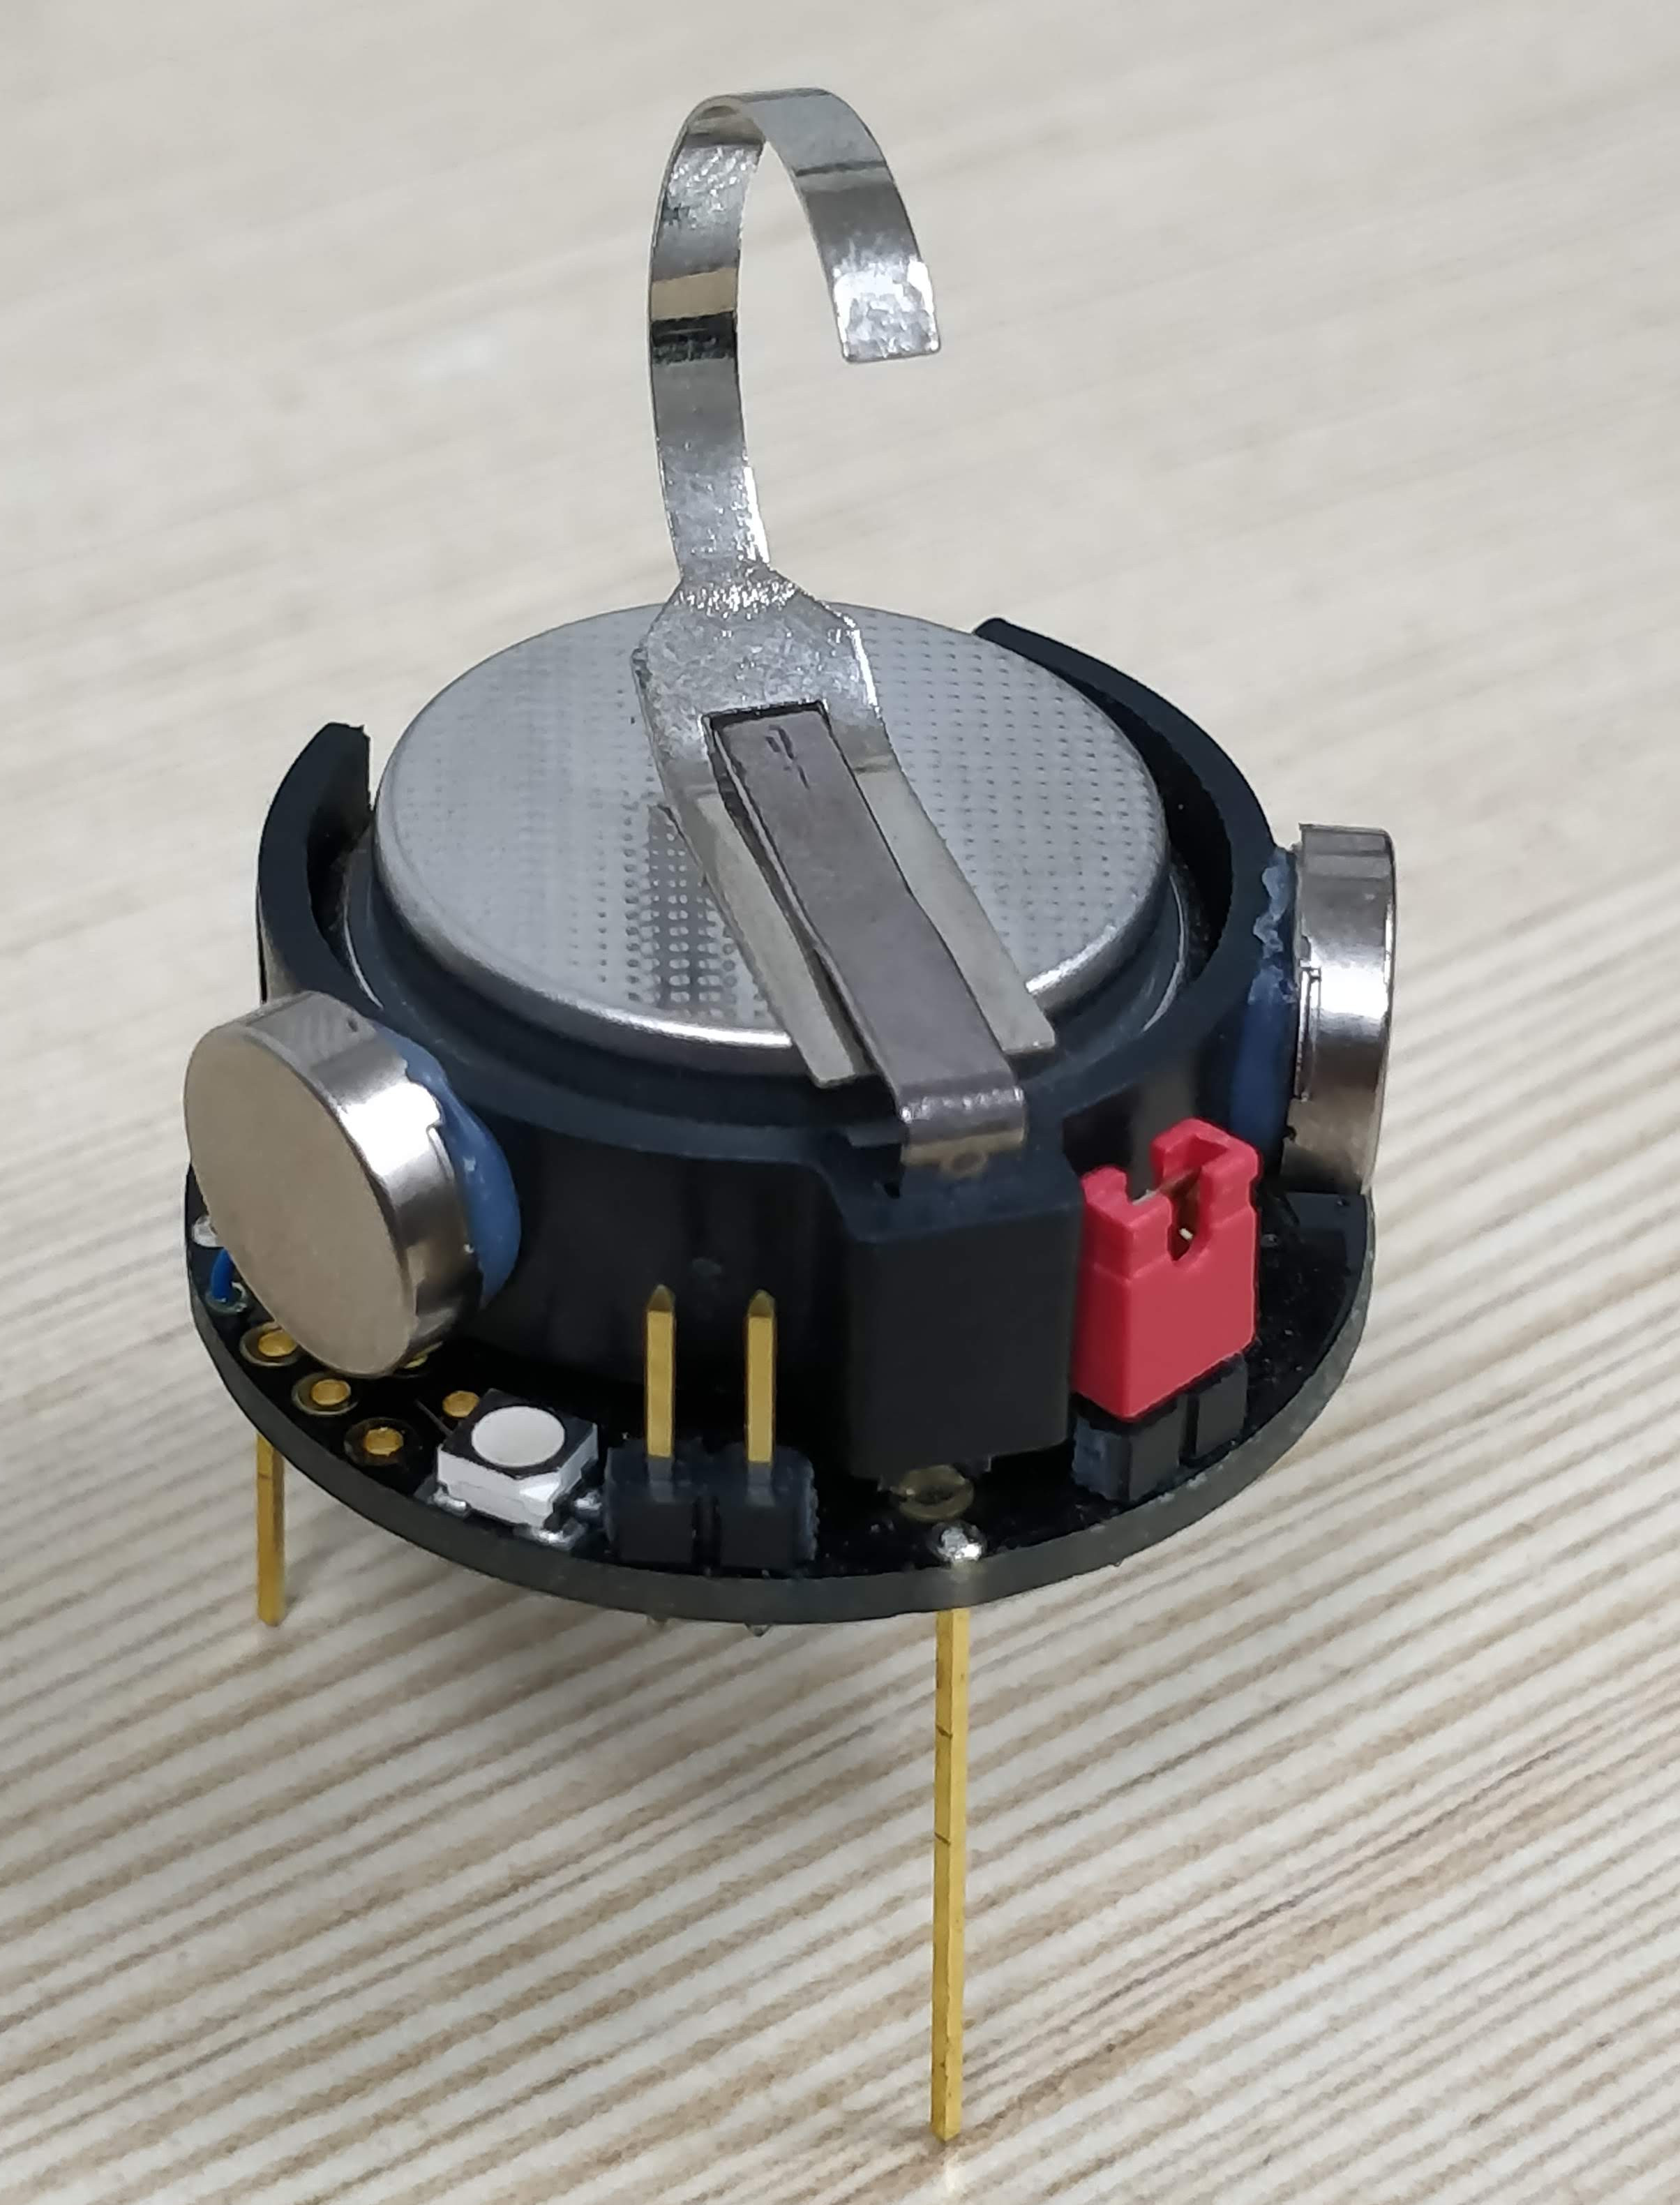
\includegraphics[scale=0.04]{images/kilobots}
		\caption{Kilobot}
		\label{fig:kilobot}
	\end{subfigure}
	\begin{subfigure}{0.45\textwidth}
		\centering
		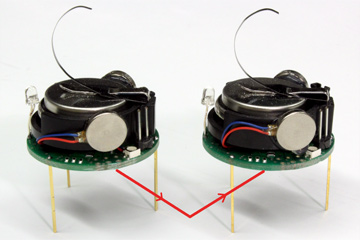
\includegraphics[scale=0.5]{images/comm}
		\caption{IR sensing (Source \cite{kilobotics_manual})}
        \label{fig:comm}
	\end{subfigure}
\end{figure}

\section{Hardware/ Software Requirement}
The required hardware and software to use the board and develop programs are described below.\\\\
Required hardware:
\begin{itemize}
\item Computer with an USB port
\item Kilobot robot
\item Over-head controller (OHC)
\item Kilobot charger
\end{itemize}

\noindent Required software:
To start programming the Kilobot with the new version from kilobotics, we  have two solutions.
\begin{itemize}
\item Online editor \url{https://www.kilobotics.com/editor}.
\item Install WinAVR and Eclipse to compile the whole library on your computer \url{https://github.com/mgauci/kilobot_notes/blob/master/eclipse_winavr_setup/eclipse_winavr_setu
p.md}. 
\end{itemize}
We have used online editor for our labs. 

\section{Over-head Controller}
To make a robot scalable to large collective sizes, all the operations of the robot must work on the collective as a whole \cite{mclurkin2006speaking}, and not require any individual attention to the robot, such as pushing a switch or plugging in a charging cable for each robot. In other words, all collective operations must be scalable. In the case of Kilobots, instead of plugging in a programming
cable to each robot in order to update its program, each can
receive a program via an IR communication channel.
This allows an overhead IR transmitter  (Figure \ref{fig:ohc}) to program all
the robots in the collective in a fixed amount of time, independent of the number of robots. 

\begin{figure}[H]
    \centering
	\fbox{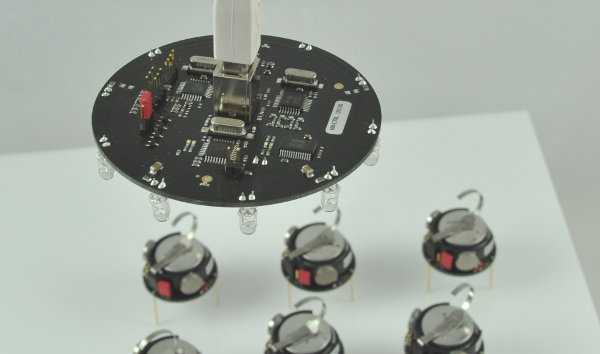
\includegraphics[scale=0.5]{images/ohc}}
	\caption{Overhead Controller (Source: \cite{kilobotics_manual})}
	\label{fig:ohc}
\end{figure}
\noindent Kilobots are unique in that they stay in ``sleep mode" until summoned by the overhead controller. A person can turn an entire swarm of Kilobots ``ON'' by sending out one signal -- as opposed to manually switching ``ON'' every robot.

\chapter{Establishing communication between two Kilobots}
Here, we will use the ability of two Kilobots to communicate with each other. We will allocate one Kilobot to be the speaker and the other Kilobot to be the listener.
\section{Speaker}
 The objective of this part is to broadcast a fixed message, and blink magenta when we transmit. Here we introduce \texttt{message\_t} data structure, and the kilo\_message\_tx lback.
\begin{itemize}
\item A Kilobot uses IR to broadcast a message within an approximately circular radius of three body lengths.

\item  Multiple robots packed closely together will interfere the IR signals. So the Kilobots use a variant of the CSMA/CD media access control method  to resolve the problems with interference.\par

Carrier-sense multiple access with collision detection (CSMA/CD) is a media access control method which uses carrier-sensing to delay transmissions until no other stations are transmitting. 
\end{itemize}

\noindent \textbf{Step 1}: Declare a variable called transmit\_msg of the structure type message\_t and add the function message\_tx() that returns the address of the message we declared (return $\And$transmit\_msg).
\newline
\newline
 \noindent \textbf{Step 2}: We will register this "callback" function in the Kilobot main loop, and every time the Kilobot is ready to send a message it will "interrupt" the main code and call the message\_tx() to get the message that needs to be sent.\par
 A callback is any executable code that is passed as an argument to other code, which is expected to call back the argument at a given time.
\begin{verbatim}
message_t transmit_msg;

message_t *message_tx() {
    return &transmit_msg;
} 

\end{verbatim}
\noindent \textbf{Step 3}:
 Use the setup() function to set the initial contents of the message and compute the message CRC value (used for error detection) through the function message\_crc(). The code below shows how to initialize a simple message. \par
 A cyclic redundancy check (CRC) is an error-detecting code which is used to detect accidental changes to raw data.
\begin{verbatim}
void setup() {
    transmit_msg.type = NORMAL;
    transmit_msg.data[0]=0;
    transmit_msg.crc = message_crc(&transmit_msg);
}
\end{verbatim}

\noindent \textbf{Step 4}:
 Now we will add some more code so that we can have the LED blink whenever the robot sends a message out. To do this we will declare a variable (often called a "boolean flag") called message\_sent. We will set this flag inside a function called message\_tx\_success() which is another callback function that only gets called when a message is finally successfully sent on a channel. Then we will clear this flag in the main loop where we will blink an LED to indicate that a message was sent. 
\begin{verbatim}
//At the top of the file, declare a "flag" for when a message is sent
int message_sent = 0;

// Add another function definition after your message_tx function
// (note that "void" means the function doesn't return any value)

void message_tx_success() {
   message_sent = 1;
}
\end{verbatim}

\noindent \textbf{Step 5}:
Then, in our program loop, write code to do this

\begin{verbatim}
// Blink led magenta when you get a message
if (message_sent == 1) {
    message_sent = 0;
    set_color(RGB(1,0,1));
    delay(100);
    set_color(RGB(0,0,0));
}
\end{verbatim}

\noindent \textbf{Step 6}:
Finally, we must register our message transmission functions with the Kilobot library as follows:
\begin{verbatim}
int main() {
    kilo_init();
    kilo_message_tx = message_tx;
    kilo_message_tx_success = message_tx_success;
    kilo_start(setup, loop);

    return 0;
}

\end{verbatim}

\begin{figure}[H]
\begin{center}
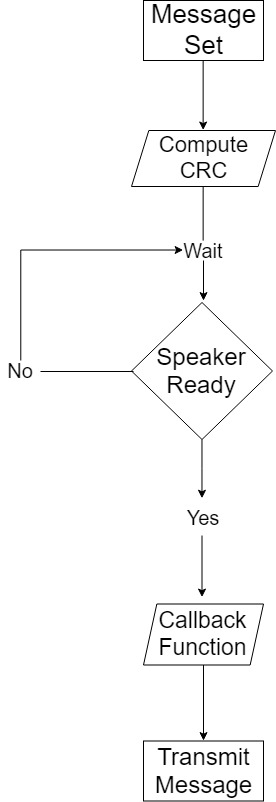
\includegraphics[scale=0.4]{speaker}
\caption{Broadcasting of a message}
\end{center}
\end{figure} 

\section{Listener}
The objective of this part is to blink yellow when a new message is received and introduce the kilo\_message\_rx callback and store incoming messages.
\newline
\newline
\noindent \textbf{Step 1}:
First declare a variable rcvd\_message of type message\_t to store any new incoming messages and a boolean variable called new\_message to indicate that a new message has been received.
\begin{verbatim}
int new_message = 0;
message_t rcvd_message;

void message_rx(message_t *msg, distance_measurement_t *dist) {
    rcvd_message = *msg;  //store the incoming message
    new_message = 1;      // set the flag to 1 to indicate that a new message arrived
}
\end{verbatim}

\noindent \textbf{Step 2}:
Check the flag in the program loop to see if a new message has arrived. If a new message has arrived, we will blink the LED yellow, and clear the flag.

\begin{verbatim}
void loop() {
    // Blink led yellow when you get a message
    if (new_message == 1) {
        new_message = 0;
        set_color(RGB(1,1,0));
        delay(100);
        set_color(RGB(0,0,0));
    }
}
\end{verbatim}
\noindent \textbf{Step 3}:
Modify our main section to register the message reception function with the Kilobot library as follows:

\begin{verbatim}
int main() {
    kilo_init();
    kilo_message_rx = message_rx;
    kilo_start(setup, loop);

    return 0;
}
\end{verbatim}
\section{Demonstration}
Video of working demo of problem statement can be accessed using link in figure \ref{fig:communication}.
\begin{figure}[H]
	\centering
	\fbox{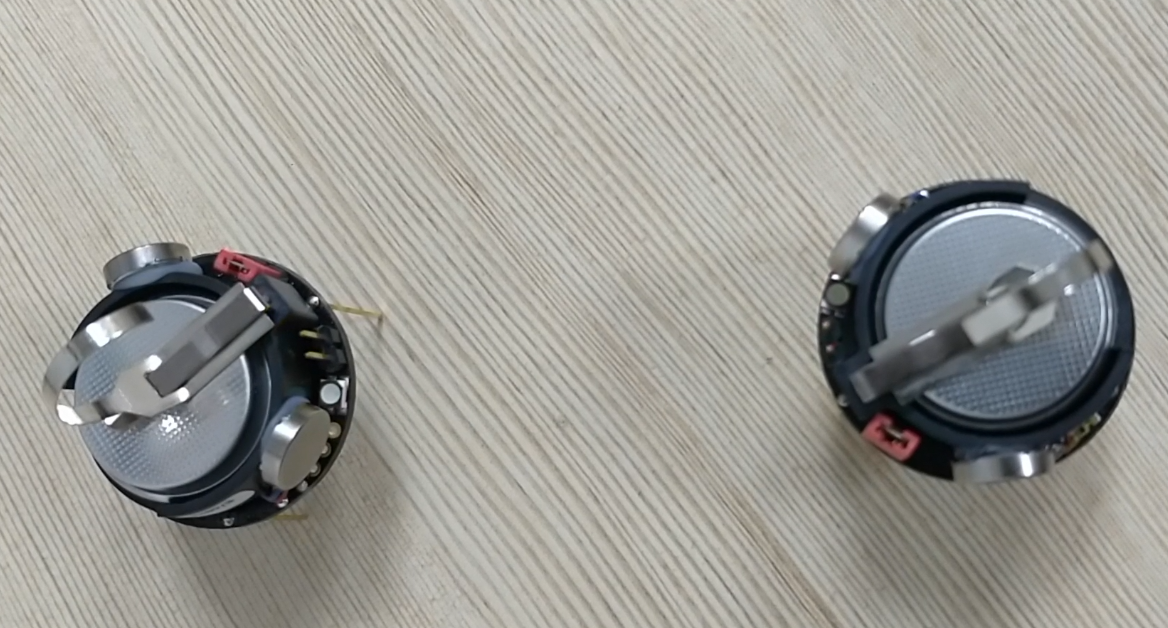
\includegraphics[scale=0.25]{images/communication}}
	\caption{\href{https://photos.app.goo.gl/h2jCY1WrUYU9xLqG8}{Communication between two Kilobots [video link]}}
	\label{fig:communication}
\end{figure}

\chapter{Orbiting of Kilobots}
Our objective is to make one Kilobot orbit a stationary Kilobot using distance estimation. We will refer to orbiting Kilobot as planet and stationary Kilobot as star. The alogrithm goes as follows:

\begin{enumerate}
    \item Place star and planet under communication link distance.
    \item If planet and star distance $<TOO\_LOW$ go to step 6, else go to step 3.
    \item If planet and star distance $<DESIRED\_DISTANCE$ go to step 4, else go to step 5.
    \item Move left. Go to step 2.
    \item Move right. Go to step 2.
    \item Move straight. Go to step 2.
\end{enumerate}
Flowchart corresponding to orbiting is illustrated in Figure \ref{fig:orbit_flowchart}

\begin{figure}
    \centering
    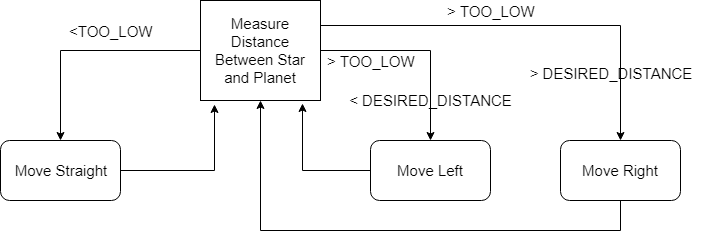
\includegraphics[scale=0.6]{images/orbiting}
    \caption{Flowchart for orbiting of kilobot}
    \label{fig:orbit_flowchart}
\end{figure}
\section{Demonstration}
Star transmits the message to planet continously while planet receives message from star and it estimates the distance between them using the strength of received signal and then accordingly it follows the algorithm.\\
Video of working demo of problem statement can be accessed using link in figure \ref{fig:orbit}.
\begin{figure}[H]
	\centering
	\fbox{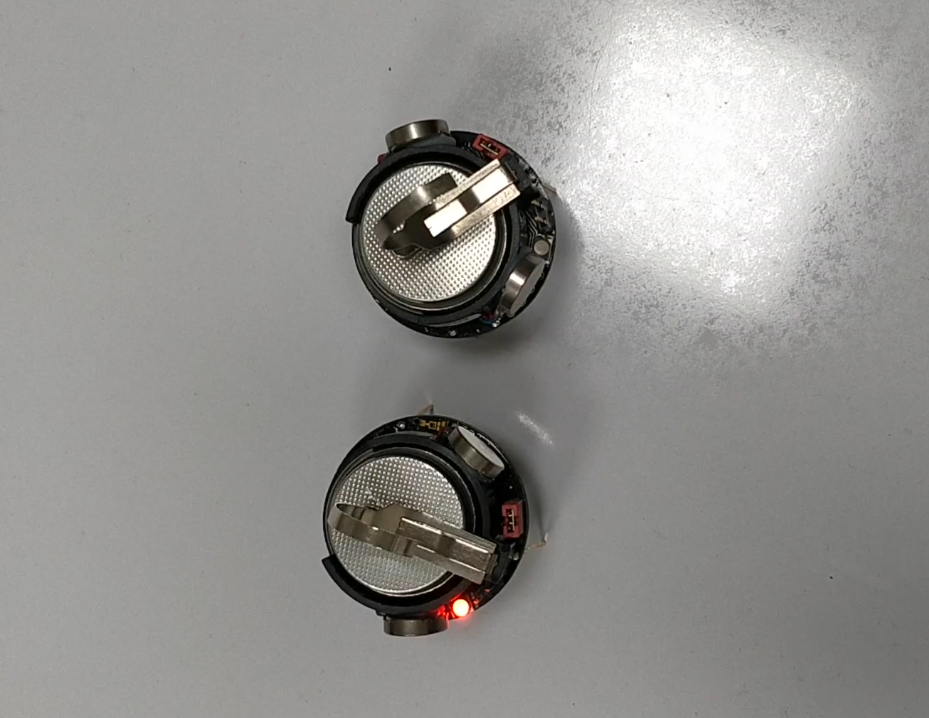
\includegraphics[scale=0.3]{images/orbit}}
	\caption{\href{https://photos.app.goo.gl/xPYoywncwhCk585X8}{Orbiting of Kilobot [video link]}}
	\label{fig:orbit}
\end{figure}
we will be using the distances of the recived message to determine how to move so you need to have estimate\textunderscore distance() in your message\textunderscore rx()\\

\chapter{Moving towards the direction of light source}
In this part, our objective is to design an algorithm so that Kilobot approaches a source of light (generated by torch light of smartphone) which may be dynamically moving with very slow speed.\\
The problem statement is similar to that of a line follower with just one onboard sensor \cite{simple-line-follower}. The algorithm for single sensor line follower goes as follows:
\begin{enumerate}
	\item Check sensor position.
	\item If sensor is on line, go to step 3 else step 4.
	\item Move right. Go to step 5.
	\item Move left.
	\item Go to step 1
\end{enumerate}
On similar lines, following a light source algorithm is implemented using flowhcart illustrated in Figure \ref{fig:move_towards_light_algorithm}.
\begin{figure}[H]
	\centering
	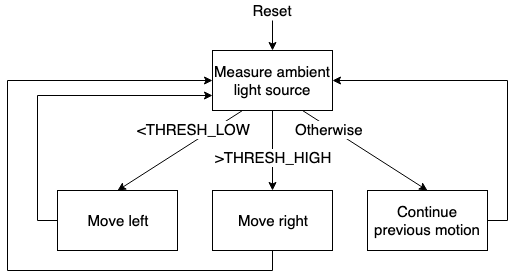
\includegraphics[scale=0.6]{images/move_towards_light_algorithm}
	\caption{Flowchart for move towards light algorithm}
	\label{fig:move_towards_light_algorithm}
\end{figure}
Abovementioned algorithm will help us understand why the robot approaches the source of light in a zig zag fashion. We cannot do significant improvement in algorithm given the limitation of onboard ambient light sensor to one.
\section{Demonstration}
Video of working demo of problem statement can be accessed using link in Figure \ref{fig:move_towards_the_light}.
\begin{figure}[H]
	\centering
	\fbox{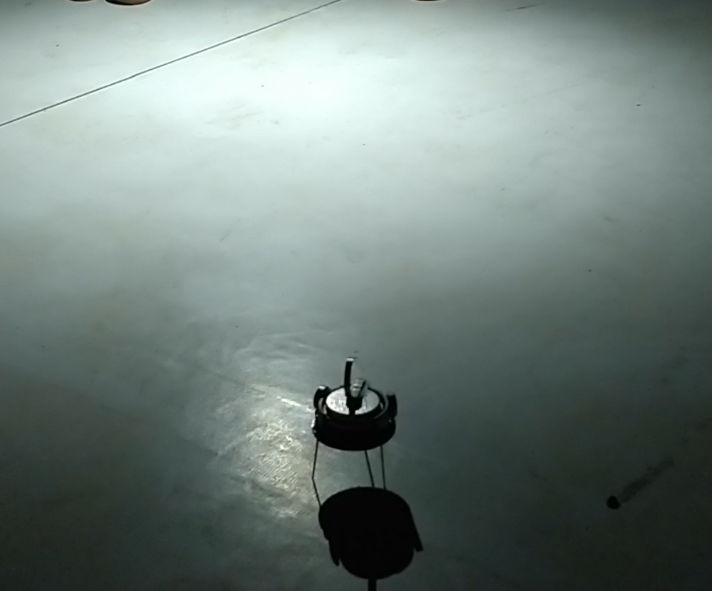
\includegraphics[scale=0.4]{images/move_towards_light}}
	\caption{\href{https://www.google.com/url?sa=j&url=https\%3A\%2F\%2Fphotos.app.goo.gl\%2FnUNghDg4nJygpzUu5&uct=1551610784&usg=G0tZGJ7iMN79F5qGk1QMw5rfodM.}{Move towards the light source [Video link]}}
	\label{fig:move_towards_the_light}
\end{figure}
Different $THRESH\_LOW$ and $THRESH\_HI$ parameters were chosen to implement hysteresis behaviour, thereby, precludingjittery motion.


\chapter{Synchronizing phase of blinking LEDs}
\textbf{Objective}: Create a logical synchronous clock between different 
robots to allow two or more Kilobots to blink an LED in unison roughly every 4 seconds \\

\noindent A large group of decentralized closely cooperating entities, commonly called a collective or \textbf{swarm}, can work together to complete a task that is beyond the capabilities of any of its individuals \cite{rubenstein2014kilobot}. Following are the three basic swarm behaviors \cite{rubenstein2014kilobot} that Kilobots have mastered: 
\begin{enumerate}
	\item  \textbf{Foraging} -- It involves commanding several robots to disperse and explore the area around them. With Kilobots, the idea is to chip away the time it takes to forage in a particular location. 
	\item  \textbf{Formation control} -- It means the ability of Kilobots to behave in unison or in a specific part of the swarm. By maintaining communication with each other, Kilobots possess a virtual bearing sensor that gives each one a realistic sense of its position in the group. 
	\item \textbf{Synchronization} -- It is often used when coordinating simultaneous actions between many entities, such as robots or sensor networks. We can  visualize this by imagining a swarm of 1,000 Kilobots, with each using its LED light to represent a pixel in a larger video that can be viewed from above. To know which color to signal at any given time, every Kilobot must be using the same clock.
\end{enumerate}
Hence, synchronization is one of the swarm behaviours which can be performed by Kilobots. It is often used when coordinating simultaneous
actions between many entities, such as robots or sensor networks.\\

\begin{figure}[H]
    \centering
	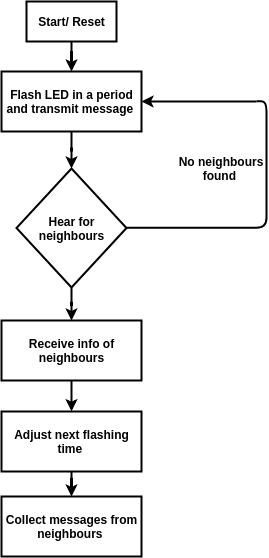
\includegraphics[scale=0.8]{images/sync-algo}
	\caption{Algorithm for synchronizing phase of blinking LEDs }
	\label{fig:sync}
\end{figure}

\noindent For our objective, we will use a method that relies on averaging. The algorithm for Synchronizing robots is given in the flowchart (Figure \ref{fig:sync}).  Each Kilobot acts as an oscillator, flashing its LED in a fixed period \texttt{P}.  At the same time, it continually transmits a message with its current position in the clock period (i.e. a value between \texttt{0} and \texttt{P}.  In the absence of any neighbors, the Kilobot will simply blink in a fixed period, like a firefly.  If the Kilobot hears neighboring Kilobots, then it receives information about their current positions in their own periods. In order to synchronize, it collects that information and uses the average to make an adjustment to its own next flashing time. The steps can be summarized as given below: \\ 

\noindent \textbf{Step 1}: Create a robot oscillator that flashes every 2 seconds.
\begin{verbatim}
#define PERIOD 64
uint32_t reset_time = 0;

// In Program Loop

if (kilo_ticks >= (last_reset + PERIOD)) {
   set LED to red
   last_reset = kilo_ticks
} else {
   turn LED off
}
\end{verbatim}

\noindent \textbf{Step  2}: Let the Kilobot continually transmit the current position of its clock within its ticking period (i.e. \texttt{kilo\_ticks - last\_reset}). Since we reset our clock every 64 ticks, this value will be less than 64. We want this value to be as accurate as possible, so we can read the clock in the \texttt{message\_tx} function. 
\begin{verbatim}
message_t message;

message_t *message_tx() {
    message.data[0] = kilo_ticks - last_reset; // current position in PERIOD
    message.crc = message_crc(&message);
    return &message;
}
\end{verbatim}

\noindent \textbf{Step 3}: Let the Kilobot collect the messages it hears from other neighbors. 
By comparing the its own current clock position to that of its neighbors (i.e. the first byte of the received message), a Kilobot can tell how much it is out of sync with its neighbors. Each time a new message arrives, the Kilobot will store the value of the adjustment to be made. Then, when the Kilobot completes its own time period and flashes, it will also make one big adjustment for next time's flash.

\begin{verbatim}
void message_rx(message_t *m, distance_measurement_t *d)
{
    int my_timer = kilo_ticks - last_reset;
    int rx_timer = m->data[0];
    int timer_discrepancy = my_timer - rx_timer;
    
    // reset time adjustment.
    reset_time_adjustment = reset_time_adjustment + 	rx_reset_time_adjustment;
}
\end{verbatim}

\section{Demonstration}
Video of working demo of problem statement can be accessed using link in Figure \ref{fig:sync_lights}.
\begin{figure}[H]
	\centering
	\fbox{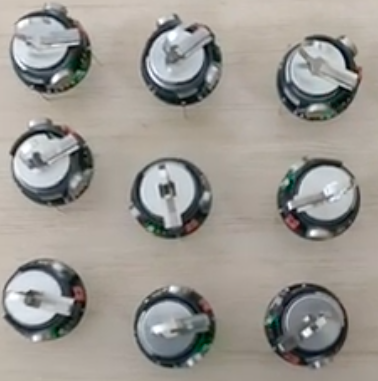
\includegraphics[scale=0.6]{images/sync_lights}}
	\caption{\href{https://photos.app.goo.gl/nvWXb5ziksYnx73s6}{Synchronizing phase of blinking LEDs}}
	\label{fig:sync_lights}
\end{figure}


\chapter{Efficient star-planet orbiting using a finite state machine}
\section{Finite state machine (FSM)}
Before discussing FSM, let us discuss the three individual terms comprising this concept viz. finite, state and machine. Finite refers to a fixed number, whereas state means the mode or position. For example, in case of a traffic light signal, we have three different states: red, yellow and green. Thus, FSM denotes a machine with fixed number of states. \cite{LL-GM-BS-rderts} views a finite state machine as:
\begin{itemize}
	\item A set of input events
	\item A set of output events
	\item A set of states
	\item A function that maps states and input to output
	\item A function that maps states and inputs to states
	\item A description of the initial state
\end{itemize}
\noindent In our case of star-planet orbiting, we model the problem as a FSM, given its suitability to modularizing different components of algorithm. Our mechanism for orbiting is very similar to those provided at Kilobotics website, and elaborately covered in details in previous chapters, although implementation using a FSM dramatically simplifies integrating macros of large size. Our main contribution in this chapter comprises of a novel and robust obstacle avoidance algorithm to prevent planet from hitting the star if it starts too close to it and also, a simple extension of existing orbiting algorithm for multiple stars setting. Both of these contributions will be dealt with extensively in coming sections. 

%\section{Discussion}
%\begin{itemize}
%\item Motor was turned on for 40ms.
%\item Spinup motor was not used as it creates chaos.
%\item Revolution time around 6 minutes.
%\item Only left, right motion was used for orbiting.
%\item Algorithm can be improved using soft delay instead of hard delay.
%\item Algorithm for escaping $too\_close$ distance worked and then stopped working suddenly.
%\item Use $max\_distance-min\_distance>some\_threshold$ to obtain orientation away from obstacle. This is more robust than checking for transition from increasing to decreasing distance.
%\item Draw flowchart for the algorithm.
%\item Motor spinup is to be used.
%\item Too close escape worked. Oscillations due to threshold on difference to check from minimum distance ($threshold\_rotate = $). New robust algorithm was used. In worst case, it will require one complete rotation.
%\item When only one distance was used, it created instability in tracking the desired orbit because planet makes only one reception and makes it decision entirely on that estimated distance.
%\item Minimum of four communication distance was used. When planet is in communication range of both the robots, it makes decision quickly but when it is in communication range of only one robot, it takes longer as it takes more time to receive 4 communication from a single star than 4 communication from two star. (Motor delay = 200, No. of communications = 4, Time = 23 minutes, 9:30 p.m.).
%\item (Motor delay = 500, No. of communications = 2, Time = 5 minutes, 9:30 p.m.). This time there is possibility of receiving communication from same star twice but that is small over successive trials.
%\item Too close escape. (Motor delay = 500, threshold = 14, radius = 65, Time = 2 minutes, 10:23 p.m.)
%\item Orbiting three stars (Time = 6 minutes, Communication = 4, Motor delay = 500).
%\item Assign different data to stars.
%\item Use float to store distance.
%\end{itemize}
\section{Flowchart}
Flowchart for orbit after escape algorithm has been divided into two parts comprising of Figure \ref{fig:orbit_after_escape1} and \ref{fig:orbit_after_escape2}. First part discusses extension of orbit algorithm for multiple star setting whereas the latter illustrates the algorithm for escaping obstacle.
\begin{figure}[H]
	\centering
	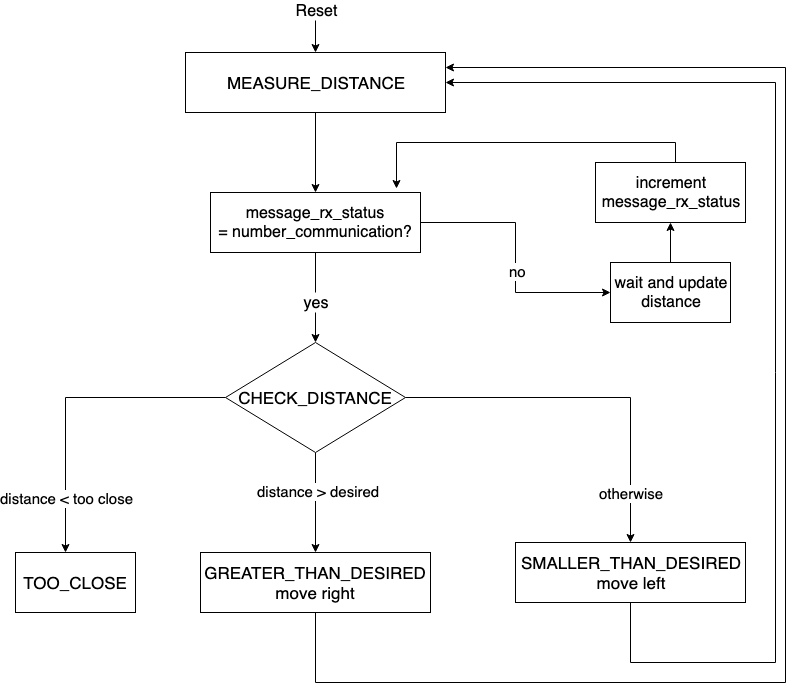
\includegraphics[scale=0.55]{star_planet_escape1}
	\caption{Flowchart for orbiting after escape algorithm (Part I)}
	\label{fig:orbit_after_escape1}
\end{figure}

In star planet orbiting algorithm, while measuring distance between stars and planet, the parameter \texttt{NUMBER\_COMMUNICATION} defines how many messages should a planet aggregate before making a decision. Accordingly, planet identifies the nearest star based on the strength of signal received in previous step. Considering the nearest star, the planet either moves left or right to maintain \texttt{DESIRED\_DISTANCE}. The parameter \texttt{message\_rx\_status} is used to keep count of successful communications.

\begin{figure}[H]
	\centering
	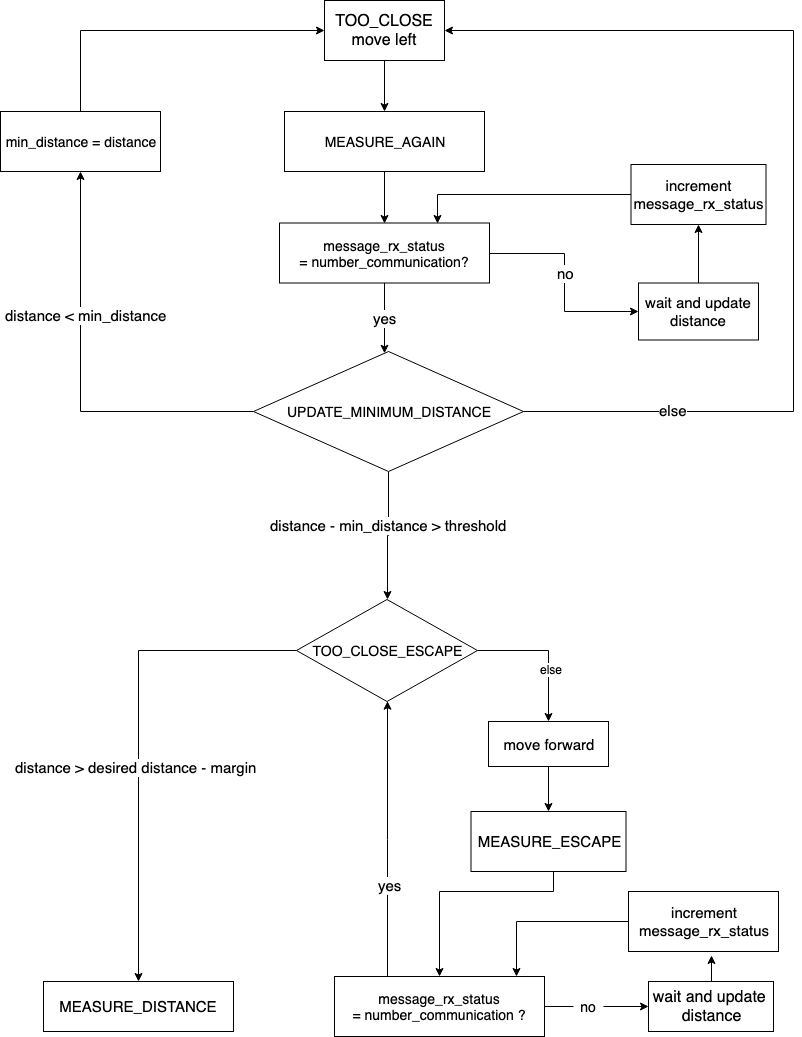
\includegraphics[scale=0.55]{star_planet_escape2}
	\caption{Flowchart for orbiting after escape algorithm (Part II)}
	\label{fig:orbit_after_escape2}
\end{figure}

The parameter \texttt{NUMBER\_COMMUNICATION} affects speed of the planet. For instance, if the number of stars in communication range is more, the planet moves faster than having only one star in communication range. This is due to the fact that it needs to receive \texttt{NUMBER\_COMMUNICATION} times of measurements  from only one star and then, decides the motion. Here are two observations, which show how the revolution time is getting varied with the number of  communications:
\begin{itemize}
	\item Motor delay = 200, Number of communications = 4, Revolution time
	      = 23 minutes
	\item Motor delay = 500, Number of communications = 2, Revolution time = 5 minutes
\end{itemize}

While escaping from \texttt{TOO\_CLOSE} region, we compare the successive distance measurements to check for the orientation of planet from star. In our early version of algorithm, we tried to detect transition of \texttt{distance} from increasing to decreasing state as the instant when planet is oriented away from star but becase of uncertainity in measurements, this led to unwanted behaviour. Hence, we decided to keep track of \texttt{minimum\_distance} from star and check for the condition \texttt{distance - min\_distance > THRESHOLD\_ROTATE} to hold. By appropriately choosing the parameter \texttt{THRESHOLD\_ROTATE}, we managed to get the final orientation of planet away from direction of star. Moreover, the modified algorithm sans over-dependence on accuracy of a single measurement, leading to filter like behaviour and an eventual robustness of solution.\\
It is worth mentioning that the robustness comes at an additional cost, which is, in worst case scenario, planet would require one complete revolution before being able to escape from \texttt{TOO\_CLOSE} region of star. For more detailed understanding of algorithm, readers are referred to code in Appendix \ref{c_orbit}.


\section{Results and Demonstration}
The caption of figure \ref{fig:efficient_star_planet_orbiting} provides link to the demonstration for orbiting of planet around the star, given star starts near the desired distance.
\begin{figure}[H]
	\centering
	\fbox{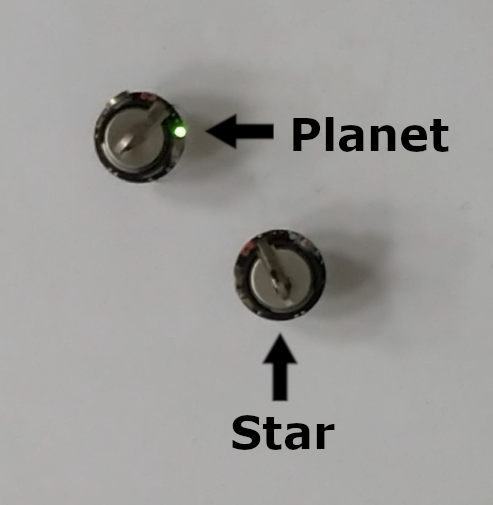
\includegraphics[width=2.5in]{images/efficient_orbiting}}
	\caption{\href{https://youtu.be/LRgOzhAJI1k}{Efficient star-planet orbiting}}
	\label{fig:efficient_star_planet_orbiting}
\end{figure}
We have hard delays in our current implementation which increases the revolution time. In future, one can replace them with soft delays to alleviate the time of revolution.

The caption of figure \ref{fig:orbit_after_escape} provides link to the demonstration of algorithm for planet to go away from too close region, which involves using a robust algorithm followed by orbiting.
\begin{figure}[H]
	\centering
	\fbox{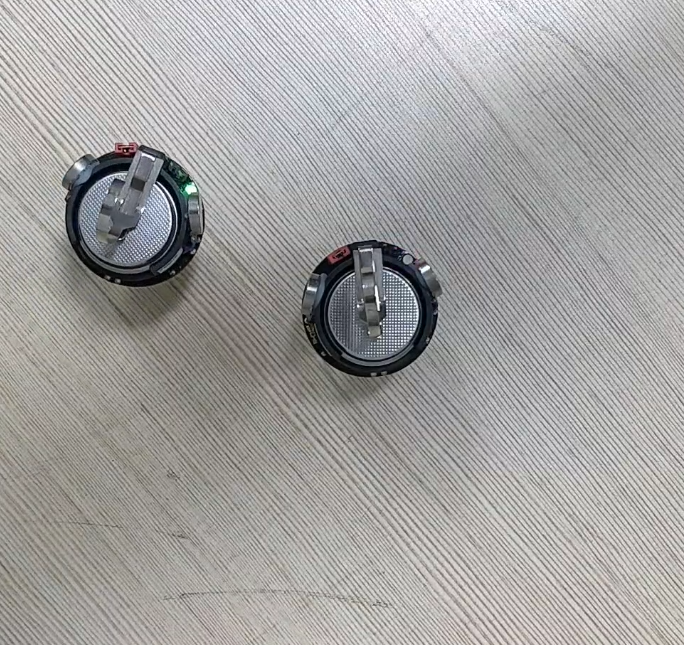
\includegraphics[width=2.7in]{images/orbit_after_escape}}
	\caption{\href{https://youtu.be/X6dGCLT0ho8}{Escaping too close region of star by planet followed by orbiting}}
	\label{fig:orbit_after_escape}
\end{figure}
It is evident from the demonstration that there is a damped oscillation before planet starts orbiting. This can be attributed to difference in centre of rotation of kilobots for clockwise and anti-clockwise turn. If it were to rotate about its centre, the oscillations would not have been as heightened as in current scenario.

The caption of figure \ref{fig:orbit_two_star_comm1} provides link to the demonstration of algorithm for planet to orbit around two stars. In this case, only one communication was used to identify minimum distance, leading to instability which can be attributed to CSMA/CD \cite{WEBOPEDIA-csma-cd} communication protocol followed by Kilobots.
\begin{figure}[H]
	\centering
	\fbox{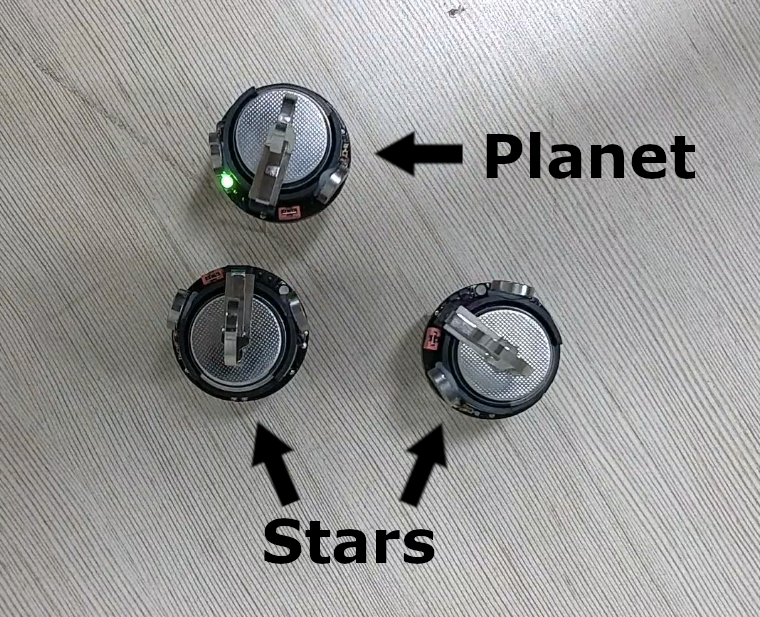
\includegraphics[width=2.7in]{images/orbit_two_stars_comm_1}}
	\caption{\href{https://youtu.be/mhW04WvGKuQ}{Orbiting of planet around two stars using single communication to estimate minimum distance leads to instability}}
	\label{fig:orbit_two_star_comm1}
\end{figure}

The caption of figure \ref{fig:orbit_two_star} provides link to the demonstration of algorithm for planet to orbit around two stars where planet uses two communications to make a descision (estimating the minimum distance).
\begin{figure}[H]
	\centering
	\fbox{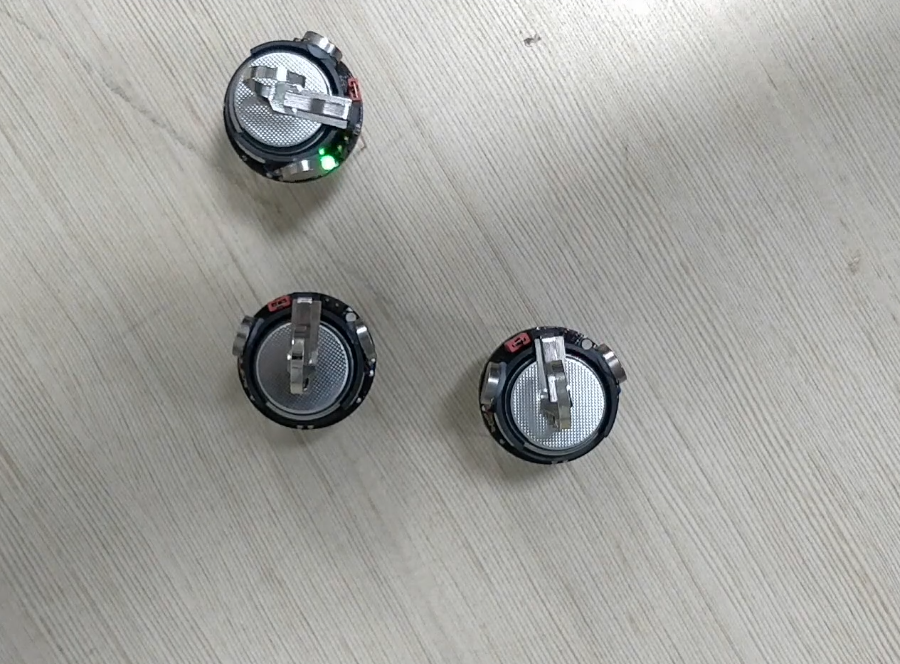
\includegraphics[width=2.7in]{images/orbit_two_stars}}
	\caption{\href{https://youtu.be/EKvty2OxXxM}{Orbiting of planet around two stars using two communications to estimate minimum distance}}
	\label{fig:orbit_two_star}
\end{figure}

The caption of figure \ref{fig:orbit_three_stars} provides link to the demonstration of algorithm for planet to orbit around three stars forming a triangle. In this case, planet uses four communications to make a decision. Though these four communications stabilize the movement of planet, it also increases  the total revolution time. 
\begin{figure}[H]
	\centering
	\fbox{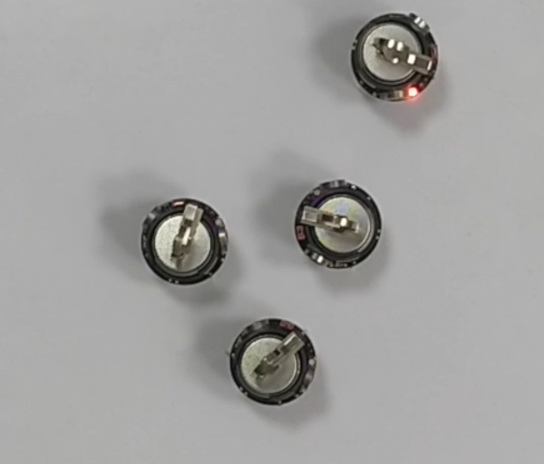
\includegraphics[width=2.7in]{images/orbiting_three_stars}}
	\caption{\href{https://youtu.be/5aZm0Os9BPc}{Orbiting of planet around three stars using four communications to estimate minimum distance}}
	\label{fig:orbit_three_stars}
\end{figure}

\section{Conclusion}
We implemented a robust algorithm for star-planet orbiting by using the concepts of FSM. This algorithm was able to prevent planet from hitting the star, even if the planet starts in the very close region of the star. Also, we observed that the movement of a planet can be stabilized by increasing the number of communications from the star. However, it will also increase the total revolution time. Also, the orientation of planets and star played a significant role. If the orientation of the planet is away from that of a star, it might take an additional turn before it begins orbiting.  


\chapter{Shape formation using Kilobots}
In this chapter, we will discuss an algorithm motivated by the work \cite{MR-AC-RN:2014} of SSL lab, Harvard University, for shape formation. Rather than implementing the entire algorithm, we will only consider a portion of it, assuming that the next robot to be placed is available near origin.
\section{Framework}
\begin{itemize}
	\item Three robots (guides) are used as reference for axis orientation.
	\item A robot (builder) participating in shape formation starts near the left of origin.
	\item In its effort to reach the desired location, builder orbits around the partial shape using the algorithm presented in last chapter.
	\item The builder stops orbiting when it reaches the desired location.
	\item Builder becomes a guide, thereby, helping the next builder.
\end{itemize}
To participate in shape formation, builders need to decide upon what global shape to form. This is achieved by sharing a shape matrix encapsulating the desired shape as an array of 5-tuple. The 5-tuple contains the following information necessary for establishing builders at desired location:
\begin{align}
	\left(
	\begin{matrix}
	Index & Neighbour_1 & Desired\ distance_1 & Neighbour_2 & Desired\ distance_2 
	\end{matrix}
	\right)
\end{align}
For forming a linear shape of width 2, the shape matrix would look like
\begin{align}
	\label{eq:shape_matrix_linear}
	\begin{bmatrix}
	3      & 1      & 1      & 2      & 1        \\
	4      & 2      & 1      & 3      & \sqrt{2} \\
	5      & 3      & 1      & 4      & 1        \\
	\cdots & \cdots & \cdots & \cdots & \cdots   
	\end{bmatrix}
\end{align}
It is important to note that we require the shape to ensure two guides for each builder node or else builder would fail to localize correctly.
\section{Flowchart}
Figure \ref{fig:fc_shape_form} explains the algorithm for shape formation. Our algorithm differs from \cite{MR-AC-RN:2014} in its implementation of shape matrix, and localization to be discussed later in next section.
\begin{figure}[H]
	\centering
	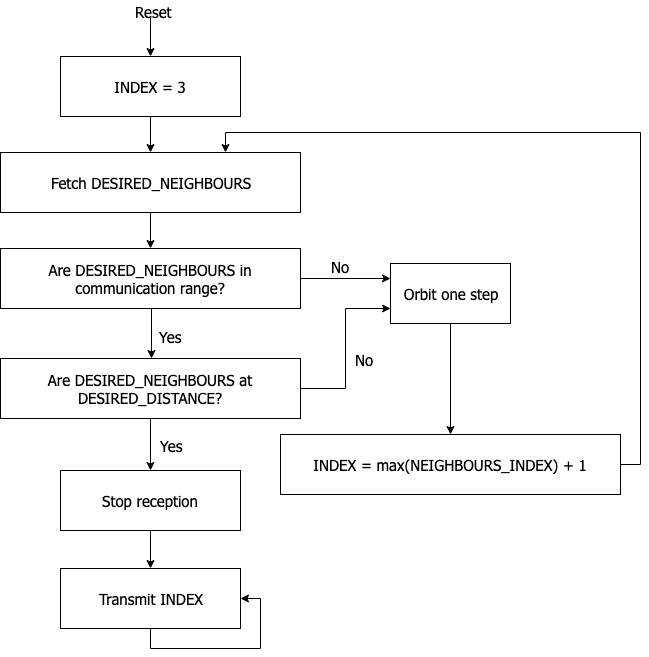
\includegraphics[scale=0.6]{images/shape_formation}
	\caption{Flowchart for shape formation algorithm}
	\label{fig:fc_shape_form}
\end{figure}

\section{Discussion}
Figure \ref{fig:shape_formation_process_1} and \ref{fig:shape_formation_process_2} helps in visualizing the shape formation process for shape matrix \eqref{eq:shape_matrix_linear}, which corresponds to a line of width 2. Black circles indicate guide robots which continuously transmit their \texttt{Index}, whereas grey circles indicate the oncoming builder robot. Shaded circle corresponds to a builder transforming into a guide. A builder is always in listener mode, whereas a guide is always in speaker mode of communication. Dotted lines trace the path of builder.

When first builder initialized with \texttt{Index=3} starts its journey, as shown in Figure \ref{fig:shape_formation_process_1}, it never faces a situation which requires \texttt{Index} update and hence, it ultimately reaches the desired location corresponding to \texttt{Index=3} and transforms into a guide robot. 
\begin{figure}[H]
	\centering
	\includegraphics[scale=0.4]{"images/shape_formation_process_1"}
	\caption{First builder taking its position}
	\label{fig:shape_formation_process_1}
\end{figure}
When second builder arrives with \texttt{Index=3}, as n in Figure \ref{fig:shape_formation_process_2}, it continues on its journey to occupy the desired location coresponding to \texttt{Index=3}, but when it comes in the communication range of new guide with \texttt{Index=3}, it realizes that it needs to update its \texttt{Index} to \texttt{4}. Following which, it travels to the desired location corresponding to \texttt{Index=4} and transforms into a guide.
\begin{figure}[H]
	\centering
	\includegraphics[scale=0.4]{"images/shape_formation_process_2"}
	\caption{Second builder taking its position}
	\label{fig:shape_formation_process_2}
\end{figure}

\section{Demonstration}
\texttt{EPSILON\_MARGIN} and \texttt{MOTOR\_ON\_DURATION} plays an essential role in determining the stability and accuracy of shape formation. For large \texttt{MOTOR\_ON\_DURATION}, it is likely for builder to go beyond its desired location and continue orbiting whereas for larger \texttt{EPSILON\_MARGIN}, we get distortion in shape. Moreover, we can not choose very small \texttt{EPSILON\_MARGIN} due to error in measurements. One way to improve accuracy of shape is by adaptively decreasing the \texttt{MOTOR\_ON\_DURATION} of builder when it comes in the comunication range of desired neighbours. The two parameters discussed are borrowed from previous chapter. For detailed understanding of these parameters, readers are motivated to go through code in Appendix \ref{c_shape_form}\\
Figure \ref{fig:shape_formation_demo} provides the link to video of shape formation in action. Shape matrix \eqref{eq:shape_matrix_linear} was fed to each builder robots to form a rectangle  breadth=2 and length=3. Values for \texttt{EPSILON\_MARGIN} and \texttt{MOTOR\_ON\_DURATION} were assigned to 5 and 500 respectively. For abovementioned values of parameters, the desired shape formation took place in roughly 10 minutes with observable distortions in shape. As the shape becomes larger and larger, accumulations of these errors could prevent a builder from localization, given our naive implementation of the algorithm. We also experimented with smaller values of \texttt{EPSILON\_MARGIN}, namely 2, but because of measurement noise, builders failed to establish themselves at desired location with large probability and continued orbiting around guides. Same observations were made for large values of \texttt{MOTOR\_ON\_DURATION}, namely 1000, as we had implemented hard delays. Although, larger values decreased the time to reach near the desired region, builders failed to localize within desired error margin. This could be attributed to large displacement being made before every localization step.
\begin{figure}[H]
	\centering
	\fbox{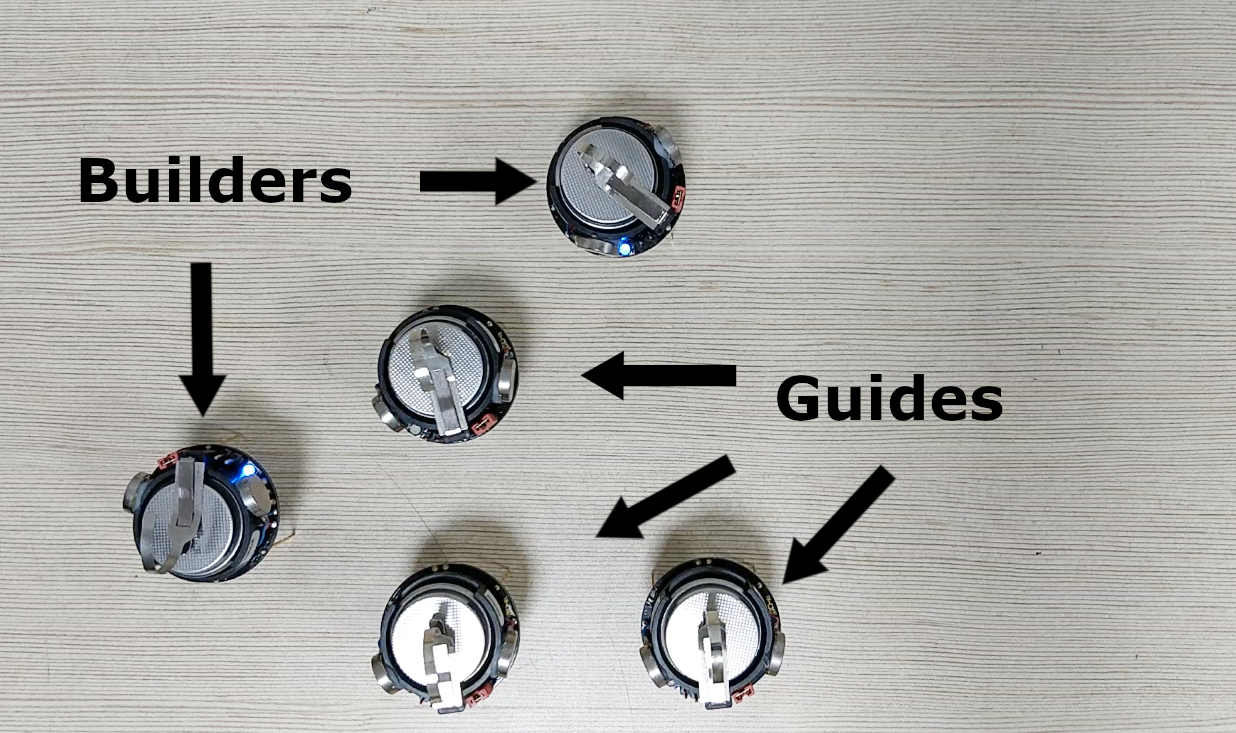
\includegraphics[width=4.5in]{images/shape_formation_demo}}
	\caption{\href{https://youtu.be/SoDq9GQvNAE}{Shape formation by kilobots (Shape: Rectangle of breadth=2 and length=3)}}
	\label{fig:shape_formation_demo}
\end{figure}
Based on our discussion, inclusion of following measures would boost the performance:
\begin{itemize}
	\item Adaptively decreasing the \texttt{MOTOR\_ON\_DURATION} as the builder reaches closer to its target location. Doing this would significantly improve the runtime of shape formation and accuracy of localization if calibrated with proper choice of \texttt{EPSILON\_MARGIN}.
	\item Conversion of hard delays to soft delays, thereby, decreasing the overall run time.
	\item Use of optimization based approach for localization to incorporate uncertainity in measurements.
\end{itemize}

\chapter{Conclusion}
During our lab work on Kilobotics, we developed essential building blocks for implementation of shape formation algorithm. In the process, we tested algorithms for efficient orbiting, algorithm for escaping an obstacle, algorithm for orbiting multiple stars, and lastly, we also implemented a rudimentary shape formation algorithm for Kilobots. There's a lot which needs to be achieved in terms of robustness in performance and integration of individual building blocks. Further, one may also pursue development of macros to generate shape matrix from a bitmap image.
\section{Acknowledgement}
We would like to thank Tejdeep Reddy for his teaching assistance and lab staffs for maintaining a healthy number of working robots. Moreover, we would like to thank Prof. Leena Vachhani for her coursework on Automation and Feedback which motivated us to approach the problem using finite state machine. Lastly, thanks to Prof. Leena Vachhani, Prof. Arpita Sinha and Adwaith Vijayakumar for their generous coperation in preponing our presentation dates. 
\appendix
\chapter{Code for orbiting after escape algorithm}
\label{c_orbit}
\lstset{
	language=C,
	numbers=left,
	stepnumber=1,
	numbersep=5pt,
	backgroundcolor=\color{white},
	showspaces=false,
	showstringspaces=false,
	showtabs=false,       
	tabsize=2,           
	captionpos=b,                   
	breaklines=true,               
	breakatwhitespace=true,       
	basicstyle=\ttfamily,
	keywordstyle=\color{blue}\ttfamily,
	stringstyle=\color{red}\ttfamily,
	commentstyle=\color{ForestGreen}\ttfamily,
	%identifierstyle=\color{Mulberry},
	morecomment=[l][\color{BrickRed}]{\#},
	numberstyle=\color{gray}
}

\lstinputlisting{code/orbit_planet_with_escape.c}
\chapter{Code for shape formation algorithm}
\label{c_shape_form}
\lstset{
	language=C,
	numbers=left,
	stepnumber=1,
	numbersep=5pt,
	backgroundcolor=\color{white},
	showspaces=false,
	showstringspaces=false,
	showtabs=false,       
	tabsize=2,           
	captionpos=b,                   
	breaklines=true,               
	breakatwhitespace=true,       
	basicstyle=\ttfamily,
	keywordstyle=\color{blue}\ttfamily,
	stringstyle=\color{red}\ttfamily,
	commentstyle=\color{ForestGreen}\ttfamily,
	%identifierstyle=\color{Mulberry},
	morecomment=[l][\color{BrickRed}]{\#},
	numberstyle=\color{gray}
}

\lstinputlisting{code/shape_formation.c}
\bibliography{anurag}{}
\bibliographystyle{ieeetr}
\end{document}
